\documentclass{article}
\usepackage{graphicx} % Required for inserting images
\usepackage{amsmath}
\title{Nonparametric Statistics Intuition}
\author{Max Lang}
\date{January 2024}

\begin{document}

\maketitle

\section{Rank Tests}
\subsection{Exchangeability}
Let's consider a set of random variables \(X_1, X_2, \ldots, X_n\). These variables are exchangeable if for any permutation \( \sigma \) from the set of all permutations \(P_n\) (which is the set of all possible ways to arrange the numbers \(1, 2, \ldots, n\)), the joint probability distribution of the permuted sequence \(X_{\sigma(1)}, X_{\sigma(2)}, \ldots, X_{\sigma(n)}\) is the same as the joint distribution of the original sequence \(X_1, X_2, \ldots, X_n\).

Intuitively, you can think of exchangeability as a "fair shuffle" of random variables. Just like shuffling a deck of cards does not change the overall makeup of the deck, permuting exchangeable random variables does not change their joint distribution. This concept often arises in contexts where the observed order of data points does not carry any inherent meaning, such as when drawing balls from an urn without looking at the colors or when surveying a group of people in random order.
\subsubsection{Difference between exchangeability and independence}
While exchangeable variables have a symmetric joint distribution, independent variables are those whose occurrence is not influenced by the occurrence of others.

Independence implies that the occurrence of one event has no effect on the probability of occurrence of another event. For two events A and B to be independent, the probability that both A and B occur should be the product of their individual probabilities: \( P(A \cap B) = P(A)P(B) \).

In the case of random variables, independence means that knowing the outcome of one variable gives no information about the outcome of another. If \(X_1, X_2, \ldots, X_n\) are independent, then the joint probability distribution factors into a product of their individual distributions:

$ P(X_1 = x_1, X_2 = x_2, \ldots, X_n = x_n) = P(X_1 = x_1)P(X_2 = x_2) \ldots P(X_n = x_n)$

Exchangeability, on the other hand, does not necessarily imply that the joint probability distribution can be factored in such a manner. Exchangeable variables can be dependent. The key with exchangeable random variables is that any subset of them has the same joint distribution as any other subset of the same size, regardless of the order. However, the occurrence of one variable in the sequence can still be dependent on the occurrence of another.

For a\textbf{ simple example}, consider a random sequence of variables representing the outcomes of flipping a fair coin: H for heads, T for tails. The sequence H, T is exchangeable because the probability of getting H followed by T is the same as getting T followed by H. However, they are also independent, because the outcome of the first flip does not affect the outcome of the second.
Now consider a different scenario: drawing balls from an urn that contains balls of different colors. Suppose we have an urn with two red balls and two blue balls. We draw two balls without replacement. The sequence of colors we draw (red, blue) is exchangeable because it has the same probability as (blue, red). However, these draws are not independent: if we know the first ball is red,
the chance of drawing a blue ball next is affected (it increases, since there are fewer red balls remaining in the urn).

Exchangeability allows for the possibility of dependence between variables, as long as the form of their joint distribution remains invariant to permutation. Independence is a stronger requirement that demands the joint distribution to be factorizable into the product of the individual distributions, which is not a requirement for exchangeability.

A key result related to exchangeable random variables is \textbf{de Finetti's theorem}, which essentially states that if an infinite sequence of random variables is exchangeable, then there is a representation of this sequence as a mixture of independent and identically distributed (i.i.d.) sequences. This theorem provides a foundational justification for Bayesian statistics and the idea of modeling unknown parameters as random variables with a prior distribution.

\subsection{Ranks}
\subsubsection{Relation between Ranks, Order Statistics and Exchangeability}
\textbf{Proposition 1.4.} If \( Z_1, \ldots, Z_N \) are exchangeable, then \( R(\mathbf{Z}) \) is uniformly distributed over \( P_N \), so that \( \Pr(R(\mathbf{Z}) = r) = \frac{1}{N!} \) for all \( r \in P_N \) and we write \( R(\mathbf{Z}) \sim U(P_N) \).

The proposition states that if a set of random variables \( Z_1, Z_2, \ldots, Z_N \) are exchangeable, then their rank \( R(\mathbf{Z}) \) is uniformly distributed over the permutation group \( P_N \), which consists of all possible orderings (permutations) of these \( N \) variables. It also states that the probability of any particular ranking \( r \) is \( 1/N! \), and this is denoted as \( R(\mathbf{Z}) \sim U(P_N) \), meaning that \( R(\mathbf{Z}) \) follows a uniform distribution over the permutations.

Intuitively, exchangeability means that the joint probability distribution of the random variables does not change when we permute the indices. In other words, the random variables are identically distributed and have the same correlation structure. Because of this, every order of these variables is equally likely.

For example, if you have three cards from a deck (say the Ace, King, and Queen of hearts), and you shuffle these three cards, the probability of any particular card being in the first, second, or third position is equal because the shuffling process does not favor any particular card or sequence. This is what it means for the cards (or random variables, in your proposition) to be exchangeable.

So, if you had to rank these cards in some way (say, based on a random drawing process), each possible ranking (Ace first, then King, then Queen, etc.) is equally likely, and there are \( 3! = 6 \) possible rankings (permutations). The uniform distribution over these 6 rankings reflects the fact that each card had an equal chance of being drawn in each position due to the shuffling process, which mirrors the concept of exchangeable random variables.

\subsection{Wilcoxon Rank Sum Test}
\begin{figure}
    \centering
    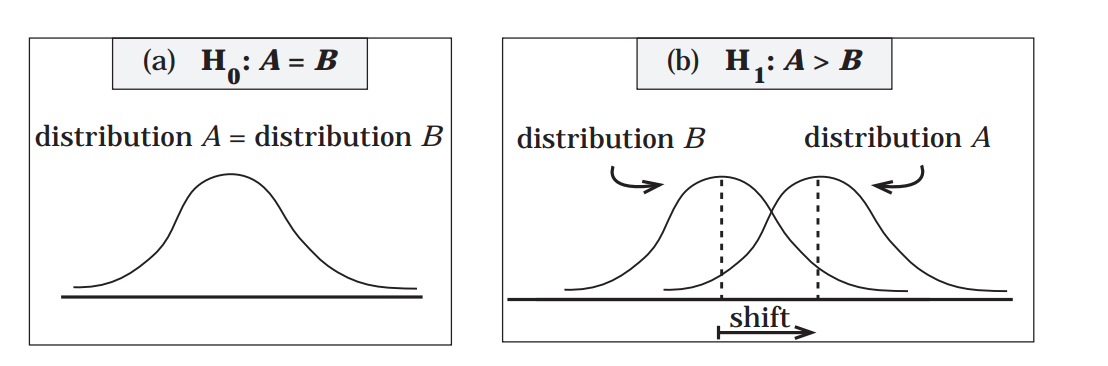
\includegraphics[width=1\linewidth]{figures/Screenshot 2024-01-17 at 19.11.14.png}
    \caption{Illustration of $H_0 : A = B$ versus $H_1 : A>B$}
    \label{fig:enter-label}
\end{figure}

\subsubsection{Decisions}

\textbf{Positive Shift (Alternative Hypothesis \( H1: \Delta > 0 \))}
This part of the test is checking whether the values in one sample (let's say Y) are generally larger than the values in the other sample (X). A "positive shift" would mean that the median of Y is greater than the median of X by some amount \(\Delta\).

- \( p^+ \) is the probability of observing a test statistic as extreme as, or more extreme than, the observed value under the null hypothesis, assuming the positive shift. If this probability is less than or equal to the significance level \( \alpha \), we reject the null hypothesis in favor of the alternative that Y tends to have larger values than X.

\textbf{Negative Shift (Alternative Hypothesis \( H1: \Delta < 0 \))}
Here, the roles are reversed; you're testing if the values in sample X are generally larger than those in sample Y.

- \( p^- \)is computed similarly to \( p^+ \), but it's for the case of a negative shift. Again, if \( p^- \) is less than or equal to \( \alpha \), you reject the null hypothesis, suggesting that X tends to have larger values than Y.

\textbf{Non-zero Shift (Alternative Hypothesis \( H1: \Delta \neq 0 \))}
This scenario is checking for any difference in medians between the two samples, regardless of direction.

- \( p^+ \) and \( p^- \) are both computed, and the smaller of the two probabilities is doubled (since we're looking at a two-tailed test here). If this doubled minimum probability is less than or equal to \( \alpha \), we reject the null hypothesis, indicating that there is a difference in medians between X and Y. The distribution of the test statistic \( W \) is symmetric around its mean under the null hypothesis, which justifies using the smaller of the two probabilities and doubling it.

In all cases, \( \alpha \) represents the significance level of the test, which is the probability threshold below which we reject the null hypothesis (often set at 0.05). Rejecting the null hypothesis implies that there is statistically significant evidence to support the alternative hypothesis – that is, there is a shift in medians between the two samples being compared.

\subsection{A normal approximation to the distribution of W}

We state this approximate test without proof. It is similar to a CLT. We have seen (in Section 1.2.3)
the distribution of \(W(R(Z))\) under the null with CDF \(G_{n,m}\) is symmetric with mean \(\mu_W = \frac{m(m+n+1)}{2}\). Its variance (PS1) is \(V_W = \frac{nm(n+m+1)}{12}\). We can see also from the example in
Figure 2 that the distribution does look quite normal, and in fact (see Gibbons and Chakraborti,
\textit{Nonparametric Statistical Inference}, CRC, (2011) for proof of this CLT) it holds that if \(W \sim G_{n,m}\) then

$$
\frac{W - \mu_W}{\sqrt{V_W}} \xrightarrow{d} N(0,1) \quad \text{as} \quad n,m \rightarrow \infty,
$$

so \(N(\mu_W, V_W)\) is an approximation to the probability mass function of the CDF \(G_{n,m}\).

\subsubsection{Continuity correction after Normal Approximation}
The continuity correction is a technique used when a discrete distribution is approximated by a continuous distribution. The most common scenario is when using the normal distribution to approximate a binomial distribution or any other discrete probability distribution in hypothesis testing, especially when calculating the p-value.

Here's an intuitive explanation:

Imagine a set of stairs, where each step represents a possible value of a discrete random variable, like the number of heads in a series of coin flips. The height of each step corresponds to the probability of that outcome. This is a discrete distribution because you can only stand on a step, not between them.

Now, suppose you want to use a ramp to approximate the steps. This ramp represents the continuous normal distribution. The ramp doesn't match the steps perfectly; it smooths out the sharp edges of the stairs into a slope.

If you're interested in the probability of being on or below a particular step (which is what a p-value represents), placing the ramp right on the steps would give you a slightly inaccurate area (probability) because the ramp would start climbing from the edge of the step, not the middle where the actual probability mass is centered.

The continuity correction adds 0.5 to the discrete value when you're on the "right side" or subtracts 0.5 when you're on the "left side." This is like shifting the ramp half a step forward or backward so it better aligns with the center of the steps. It adjusts the approximation so that the area under the curve (the ramp) more accurately reflects the sum of the probabilities of the steps up to that point.

For example, if you want to approximate the probability of observing 3 heads out of 10 flips (using a binomial distribution), you would look at the value of the normal distribution at 3.5 instead of 3. This gives you the probability of observing 'up to and a little beyond' 3 heads, which compensates for the fact that in the discrete case, exactly 3 heads is one specific outcome, whereas the continuous distribution is smooth and doesn't have such exact cut-offs.

As a further illustration, consider a binomial distribution with parameters \( p = 0.5 \) and \( n = 20 \).
Now, we try to approximate that with a normal distribution with mean \( np \) and variance
\( n(p)(1 - p) \). We use continuity corrections \( 0 \) (no correction), \( 0.25 \), \( 0.5 \), and \( 0.75 \). In the below
graph the coloured lines are the corresponding densities of the normal distribution.

\begin{figure}
    \centering
    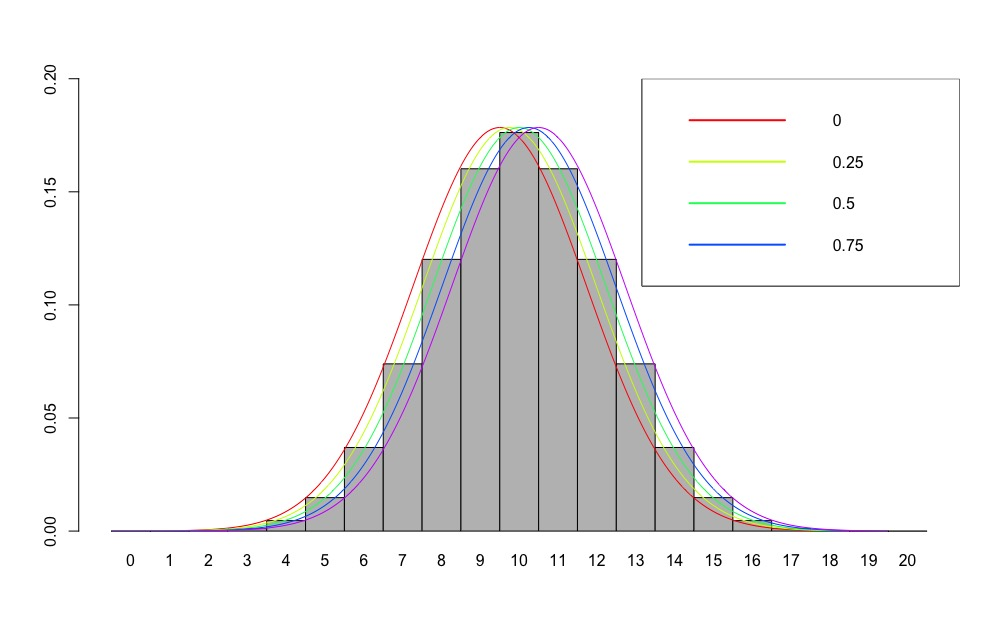
\includegraphics[width=1\linewidth]{figures/gJSmv.jpg}
    \label{fig:enter-label}
\end{figure}
As you can see, the one with continuity correction 0.5 seems to "fit best".

Now, let us look at an asymmetric example with $p =0.2$.
\begin{figure}
    \centering
    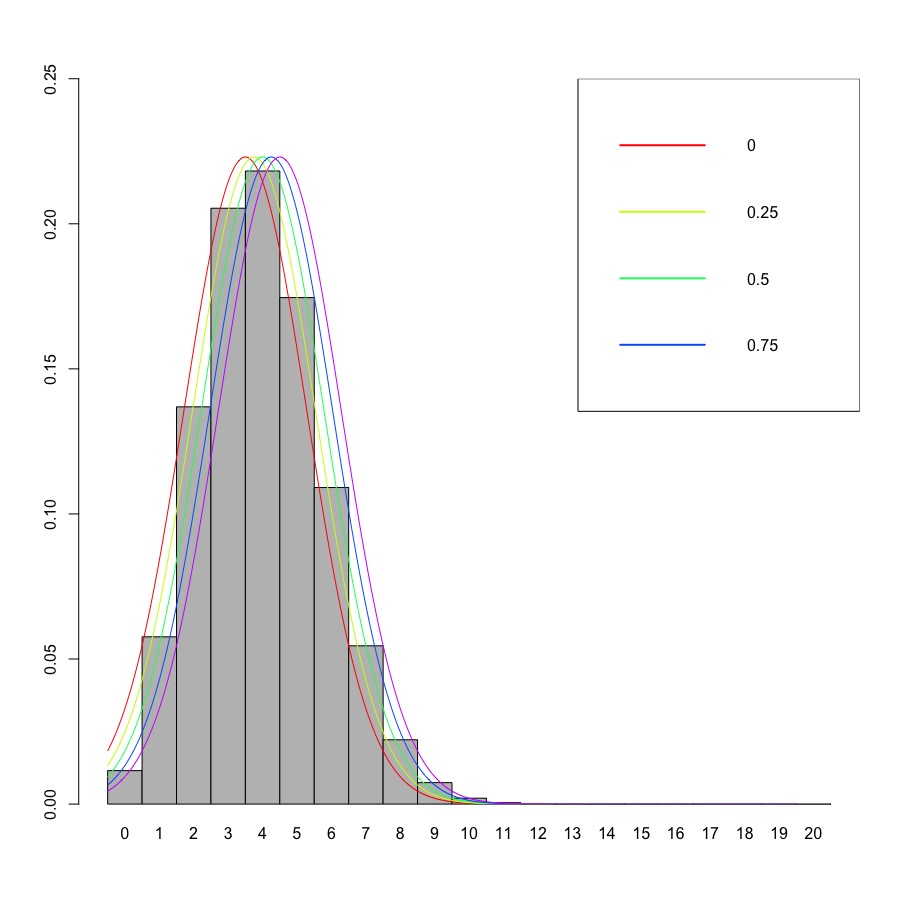
\includegraphics[width=1\linewidth]{figures/oChLi.jpg}
    \label{fig:enter-label}
\end{figure}
In order to get the best normal approximation, we need to include the area under the normal curve between 8.5 and 11.5. This use of half-integers is sometimes called a 'continuity correction. The relevant histogram bars are the ones centered at 9, 10, and 11.
\begin{figure}
    \centering
    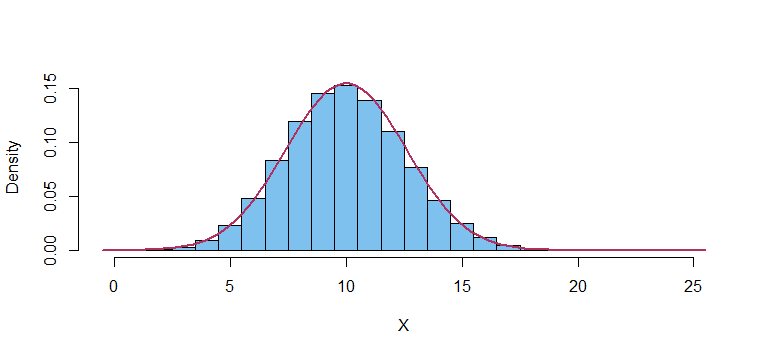
\includegraphics[width=1\linewidth]{figures/7Az90.png}
    \label{fig:enter-label}
\end{figure}


\end{document}
